% One-at-a-time term ablation of Eq. (1) -- Fig. 2.
% Bar values are read from risk_ablation_data.tex, which is generated by
%   npx tsx scripts/risk-decomposition.ts scripts/eval-heldout-full-gptoss120b.json \
%       --ablation-tex=../paper/figures/risk_ablation_data.tex
% Do not type values here.
% AUTO-GENERATED by autoops_ai/scripts/risk-decomposition.ts -- do not edit.
% Source: eval-heldout-full-gptoss120b.json (one-at-a-time term ablation of Eq. 1)
\def\ablationN{100}
\def\ablationRows{
  Blast radius/100,
  Severity/23,
  Confidence/16,
  Rollback/16,
  Template source/0,
  Trusted memory/0,
  Memory hit/0}
%
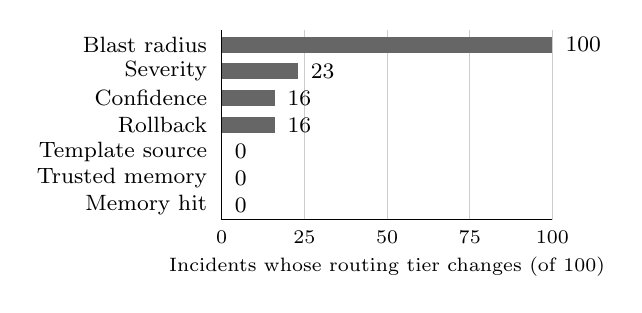
\begin{tikzpicture}[x=0.042cm, y=-0.34cm, font=\footnotesize]
  % gridlines and x axis
  \foreach \t in {0,25,50,75,100} {
    \draw[black!20, line width=0.3pt] (\t,0.45) -- (\t,7.55);
    \node[anchor=north, font=\scriptsize] at (\t,7.6) {\t};
  }
  \draw[line width=0.4pt] (0,7.55) -- (100,7.55);
  \node[anchor=north, font=\scriptsize] at (50,8.55)
    {Incidents whose routing tier changes (of \ablationN)};
  % bars with direct count labels
  \foreach \lab/\val [count=\i] in \ablationRows {
    \node[anchor=east] at (-1.5,\i) {\lab};
    \fill[black!60] (0,\i-0.3) rectangle (\val,\i+0.3);
    \node[anchor=west] at (\val+1,\i) {\val};
  }
  \draw[line width=0.4pt] (0,0.45) -- (0,7.55);
\end{tikzpicture}%
